\documentclass[../Calculus_\Roman{3}]{subfiles}

\begin{document}
	\section{Three-Dimensional Coordinate Systems}
		Any point in a plane can be represented as an ordered pair of real numbers. Because this uses two numbers, a plane is called two-dimensional. To locate a point in space, a triplet of real-numbers is required.
		\subsection*{3D Space}
			\addcontentsline{toc}{subsection}{3D Space}
			Before points can be represented in 3D space, a fixed point $O$ (the origin) and three perpendicular lines that pass through it, called the \textbf{coordinate axes}. These axes are labeled the $x$-, $y$-, and $z$-axes. In general, the former two are horizontal while the third is vertical. The direction of the $z$-axis is determined by the \textbf{right-hand rule}. Curling the fingers of the right hand from the positive $x$-axis to the positive $y$-axis, the thumb will point in the direction of the positive $z$-axis. \\
			The three coordinate axes determine the three \textbf{coordinate planes}.
			\[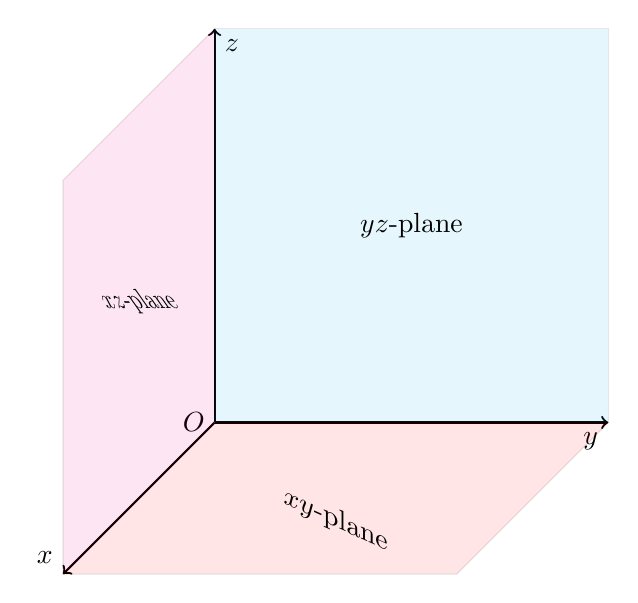
\begin{tikzpicture}[xscale = 5, yscale = 5]
				\coordinate (O) at (0, 0, 0) node[anchor = east]{$O$};
				\draw[thick, ->] (0, 0, 0) -- (1, 0, 0) node[anchor = north east]{$y$};
				\draw[thick, ->] (0, 0, 0) -- (0, 1, 0) node[anchor = north west]{$z$};
				\draw[thick, ->] (0, 0, 0) -- (0, 0, 1) node[anchor = south east]{$x$};
				\draw[fill = cyan, opacity = 0.1] (0, 0, 0) -- (1, 0, 0) -- (1, 1, 0) -- (0, 1, 0);
					\node at (0.5, 0.5, 0) {$yz$-plane};
				\draw[fill = magenta, opacity = 0.1] (0, 0, 0) -- (0, 1, 0) -- (0, 1, 1) -- (0, 0, 1);
					\node[xslant = -0.7, xscale = 0.7] at (0, 0.5, 0.5) {$xz$-plane};
				\draw[fill = red, opacity = 0.1] (0, 0, 0) -- (0, 0, 1) -- (1, 0, 1) -- (1, 0, 0);
					\node[below, yslant = -0.45] at (0.5, 0, 0.5) {$xy$-plane};
			\end{tikzpicture}\]
			Three planes divided space into eight \textbf{octants}. Illustrated above are the positive $xz$-, $yz$-, and $xy$-planes, constituting the \textbf{first octant}. \\
			A point's \textbf{coordinates} are an ordered triple of real numbers. A point's \textbf{projection} onto a plane is the point with two of the same coordinates, the third becoming 0.
			\[\begin{array}{|c|c|c|c|}\hline
				\text{Plane} & xy & yz & xz \\\hline
				(a, b, c) & (a, b, 0) & (0, b, c) & (a, 0, c) \\\hline
			\end{array}\]
			The set of all ordered triples is the cartesian product of three sets of all real numbers, denoted appropriately by $\mathbb{R}^3$ and defined as
			\[\mathbb{R}^3 = \mathbb{R} \times \mathbb{R} \times \mathbb{R} = \{(x, y, z) \mid x, y, z \in \mathbb{R}\}\]
			A one-to-one correspondence between points in space and ordered triples in $\mathbb{R}^3$ is a \textbf{three-dimensional coordinate system}. It should be noted that the first octant can be described as the set of points for which all coordinates are positive.
			\subsection*{Distances and Spheres}
				\addcontentsline{toc}{subsection}{Distances and Spheres}
			\callout{17}{
				\paragraph{Distance Formula in Three Dimensions} The distance $|P_1P_2|$ between points $P_1(x_1, y_1, z_1)$ and $P_2(x_2, y_2, z_2)$ is
				\[|P_1P_2| = \sqrt{(x_2 - x_1)^2 + (y_2 - y_1)^2 + (z_2 - z_1)^2}\]
			}
			\callout{17}{
				\paragraph{Equation of a Sphere}
					The equation of a sphere with center $(h, k, l)$ and radius $r$ is
					\[(x - h)^2 + (y - k)^2 + (z - l)^2 = r^2\]
			}
		\section{Vectors}
			The term \textbf{vector} is used to indicate a quantity with both magnitude and direction.
			\subsection*{Geometric Description of Vectors}
				\addcontentsline{toc}{subsection}{Geometric Description of Vectors}
				A vector is often represented by an arrow, the length of which represents its magnitude. A vector is denoted by a letter in boldface (\textbf{v}) or with an arrow above a letter ($\vec{v}$). \\
				A \textbf{displacement vector} is a vector representing how something is displaced from its \textbf{initial point} (tail) to its \textbf{terminal point} (tip).
				\[\begin{tikzpicture}
					\draw[thick, ->] (0, 0) node[anchor = north east]{$A$} -- node[anchor = south east]{$\vec{v}$} ++ (2, 1.5) node[anchor = south west]{$B$};
					\draw[thick, ->] (3, 0.25) node[anchor = north east]{$C$} -- node[anchor = south east]{$\vec{u}$} ++ (2, 1.5) node[anchor = south west]{$D$};
				\end{tikzpicture}\]
				In the above figure, vector $\vec{v}$ has initial point $A$ and terminal point $B$. This can be indicated by writing $\vec{v} = \Vec{AB}$. If $AB = CD$ and the angles relative to the same axis are equal, then the $\vec{v}$ and $\vec{u}$ are \textbf{equivalent} (or \textbf{equal}). \\
				The only vector without a direction is the \textbf{zero vector}, denoted by $\vec{0}$, which has length 0. \\
				The sum of two vectors can be denoted with the initial point of the first and the terminal point of the second. \\
				\[\begin{tikzpicture}
					\draw[thick, ->, color = red] (0, 0) node[anchor = north east]{$A$} -- (1.49, 1.75) node[anchor = south west]{C};
					\draw[thick, ->] (0, 0) -- (2.5, 1) node[anchor = west]{$B$};
					\draw[thick, ->] (2.5, 1) -- (1.51, 1.75);
					\node[] at (6, 1){\small$\Vec{AB} + \Vec{BC} = \Vec{AC}$};
				\end{tikzpicture}\]
				To add vectors, the one's tail can be moved to the other's tip and the resultant terminal point found.
				\callout{17}{\paragraph{Definition of Vector Addition} The sum of two vectors position such that the initial point of one is the terminal point of the other is the vector from the initial point of the first to the terminal point of the second.}
				The definition of vector addition is sometimes referred to as the \textbf{Triangle Law}.
				\[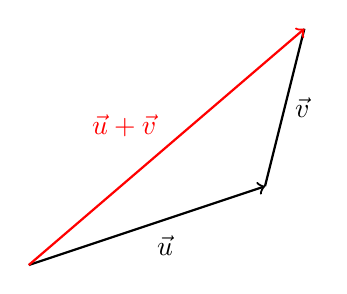
\begin{tikzpicture}
					\draw[thick, ->] (0, 0) -- node[anchor = north west]{$\vec{u}$} ++ (3, 1);
					\draw[thick] (3, 1) -- node[anchor = west]{$\vec{v}$} ++ (0.5, 2);
					\draw[thick, ->, color = red] (0, 0) -- node[anchor = south east]{$\vec{u} + \vec{v}$} ++ (3.5, 3); 
				\end{tikzpicture}\]
				Doing the opposite addition results in the same resultant vector. This is made visible b y the \textbf{Parallelogram Law}.
				\[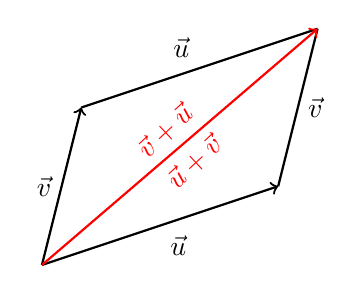
\begin{tikzpicture}
					\draw[thick, ->] (0, 0) -- node[anchor = north west]{$\vec{u}$} ++ (3, 1);
					\draw[thick] (3, 1) -- node[anchor = west]{$\vec{v}$} ++ (0.5, 2);
					\draw[thick, ->] (0, 0) -- node[anchor = east]{$\vec{v}$} (0.5, 2);
					\draw[thick] (0.5, 2) -- node[anchor = south east]{$\vec{u}$} ++ (3, 1);
					\draw[thick, ->, color = red] (0, 0) -- node[anchor = south, rotate = 43]{$\vec{v} + \vec{u}$} node[anchor = north, rotate = 43]{$\vec{u} + \vec{v}$} ++ (3.5, 3);
				\end{tikzpicture}\]
				A \textbf{scalar} is a number that is not a vector.
				\callout{17}{\paragraph{Definition of Scalar Multiplication} The \textbf{scalar multiple} $c\vec{v}$ of a scalar $c$ and a vector $\vec{v}$ is a vector of length $|c||\vec{v}|$ and whose direction is the same as $\vec{v}$ is $c > 0$ and in the opposite direction if $c < 0$. If $c = 0$ or $\vec{v} = \vec{0}$, then $c\vec{v} = \vec{0}$.}
				The \textbf{negative} of a vector $\vec{v}$, denoted by $-\vec{v}$, is the scalar multiple of the $\vec{v}$ and $-1$. \\
				The \textbf{difference} $\vec{u} - \vec{v}$ is the sum of $\vec{u}$ and $-\vec{v}$.
				\[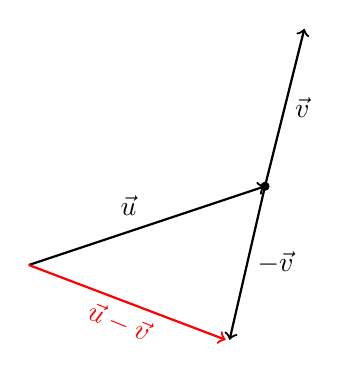
\begin{tikzpicture}
					\draw[thick, ->] (0, 0) -- node[anchor = south east]{$\vec{u}$} ++ (3, 1);
					\filldraw (3, 1) circle (0.5mm);
					\draw[thick, ->] (3, 1) -- node[anchor = west]{$\vec{v}$} ++ (0.5, 2);
					\draw[thick, ->] (3, 1) -- node[anchor = west]{$-\vec{v}$} ++(-0.45, -1.95);
					\draw[thick, ->, color = red] (0, 0) -- node[anchor = north, rotate = -22]{$\vec{u} - \vec{v}$} (2.5, -0.95);
				\end{tikzpicture}\]
				A vector can be treated algebraically using \textbf{components}, which are the difference between the initial and terminal points in a dimension. The components of a vector $\vec{u}$ in 2 dimension and a vector $\vec{v}$ in 3 can be denoted as such:
				\begin{align*}
					\vec{u} &= \langle u_1, u_2 \rangle & \vec{v} &= \langle v_1, v_2, v_3 \rangle
				\end{align*}
				Geometric vectors can be though of as \textbf{representation} of algebraic vectors.
				\callout{17}{The representation of a vector with initial and terminal points is \[\langle \Delta x, \Delta y, \Delta z \rangle\]}
				The \textbf{magnitude/length} of a vector, denoted $|\vec{v}|$ or $||\vec{v}||$ for a vector $\vec{v}$, is the length of any of its representations. This can be computed in $n$ dimensions using the distance formula:
				\[|\vec{v}| = \sqrt{\sum_{i = 1}^n v_i^2}\]
				Vectors can be added or subtracted algebraically by performing the desired operation their corresponding components.
				\[\vec{u} \pm \vec{v} = \langle u_1 \pm v_1, u_2 \pm v_2, \ldots, u_n \pm v_n \rangle\]
				The scalar multiple of a vector can be found by multiplying each of its components by the scalar.
				\[c\vec{v} = \langle cv_1, cv_2, \ldots, cv_n \rangle\]
				The set of all $n$-dimensional vectors is denoted by $V_n$.
				An $n$-dimensional vector is an $n$-tuple of real numbers, which are the vector's components.
				\callout{17}{
					\paragraph{Properties of Vectors}
						If $\vec{a}$, $\vec{b}$, and $\vec{c}$ are vectors in $V_n$ and $c$ and $d$ are scalars, then	
						\begin{align*}
							\vec{a} + \vec{b} &= \vec{b} + \vec{a} &
								\vec{a} + (\vec{b} + \vec{c}) &= (\vec{a} + \vec{b}) + \vec{c} \\
							\vec{a} + \vec{0} &= \vec{a} &
								\vec{a} + (-\vec{a}) &= \vec{0} \\
							c(\vec{a} + \vec{b}) &= c\vec{a} + c\vec{b} &
								(c + d)\vec{a} &= c\vec{a} + d\vec{a} \\
							(cd)\vec{a} &= c(d\vec{a}) &
								1\vec{a} &= \vec{a}
						\end{align*}
				}
				A vector can be denoted in \textbf{unit-vector notation} as the sum of scalar multiples of \textbf{standard basis vectors} defined as such:
				\begin{align*}
					\vi &:= \langle 0, 0, 1 \rangle &
						\vj &:= \langle 0, 1, 0 \rangle &
						\vk &:= \langle 0, 0, 1 \rangle
				\end{align*}
				A vector can therefore be rewritten using its components as such:
				\[\vec{v} = \langle v_x, v_y, v_z \rangle = v_x\vi + v_y\vj + v_z\vk\]
				A \textbf{unit vector} is a vector of length 1. The standard basis vectors are unit vectors in the directions of the axes. A unit vector $\vec{u}$ in the same direction as a vector $\vec{v}$ is
				\[\vec{u} = \frac{\vec{a}}{|\vec{a}|}\]
				The angle $\theta$ between a two-dimensional vector $\vec{v}$ and the positive $x$-axis can be calculated using inverse tangent:
				\[\theta = \arctan\left(\frac{v_y}{v_x}\right)\]
				This can be used to find the components of a vector of a given magnitude $r$ and direction $\theta$.
			\section{The Dot Product}
				\callout{17}{
					\paragraph{Definition of the Dot Product}
						The dot product of two vectors in $V_n$ is the sum of the products of their corresponding components.
						\[\vec{u} \cdot \vec{v} = \sum_{i = 1}^n u_iv_i\]
				}
				The dot product of two vectors is a real number. As such, the dot product is sometimes referred to as the \textbf{scalar/inner product}. \\
				\callout{17}{
					\paragraph{Properties of the Dot Product}
						If $\vec{a}$, $\vec{b}$, and $\vec{c}$ are vectors in $V_n$ and $c$ is a scalar, then
							\begin{align*}
								\vec{a} \cdot \vec{a} &= |\vec{a}|^2 &
									\vec{a} \cdot \vec{b} &= \vec{b} \cdot \vec{a} \\
								\vec{a} \cdot (\vec{b} + \vec{c}) &= \vec{a} \cdot \vec{b} + \vec{a} \cdot \vec{c} &
									(c\vec{a}) \cdot \vec{b} &= c(\vec{a} \cdot \vec{b}) = \vec{a} \cdot (c\vec{b}) \\
								\vec{0} \cdot \vec{a} &= 0
							\end{align*}
				}
				\callout{17}{
					If $\theta$ is the angle between vectors, $\vec{a}$ and $\vec{b}$, then
						\[\vec{a} \cdot \vec{b} = |\vec{a}||\vec{b}|\cos\theta\]
					Rewritten for $\theta$, it can be said that
					\[\cos\theta = \frac{\vec{a} \cdot \vec{b}}{|\vec{a}||\vec{b}|}\]
				}	
			\section{The Cross Product}
				A \textbf{determinant of order 2} is defined as the difference between the products of the diagonal terms and is denoted as such:
					\[\begin{vmatrix} a & b \\ c & d \end{vmatrix} = ad - bc\]
					A \textbf{determinant of order 3} can be defined in terms of second-order determinants.
					\begin{align*}
						\begin{vmatrix} 
							a_1 & a_2 & a_3 \\ 
							b_1 & b_2 & b_3 \\ 
							c_1 & c_2 & c_3 
						\end{vmatrix} &=
						a_1\begin{vmatrix}
							b_2 & b_3 \\
							c_2 & c_3
						\end{vmatrix} -
						a_2\begin{vmatrix}
							b_1 & b_3 \\
							c_1 & c_3
						\end{vmatrix} +
						a_3\begin{vmatrix}
							b_1 & b_2 \\
							c_1 & c_2
						\end{vmatrix} \\
							&= a_1b_2c_3 - a_1b_3c_2 - a_2b_1c_3 + a_2b_3c_2 + a_3b_1c_2 - a_3b_2c_1
					\end{align*}
					\callout{17}{
						\paragraph{Definition of the Cross Product}
							The \textbf{cross product} of two three-dimensional vectors $\vec{a}$ and $\vec{b}$ is 
							\[
								\vec{u} \times \vec{v} = 
									\begin{vmatrix}
	 									\vi & \vj & \vk \\
	 									u_1 & u_2 & u_3 \\
	 									v_1 & v_2 & v_3
							 		\end{vmatrix} =
							 		\langle u_2v_3 - u_3v_2, u_3v_1 - u_1v_3, u_1v_2 - u_2v_1 \rangle
							\]
					}
					The cross product of two vectors is orthogonal to both. \\
					The magnitude of the cross product of two vectors $\vec{u}$ and $\vec{v}$ with angle $\theta$ between them is $\vec{0}$.
						\[|\vec{u} \times \vec{v}| = |\vec{u}||\vec{v}|\sin\theta\]
					\callout{17}{
							Two vectors are parallel if and only if their cross product is equal to zero.
								\[\vec{u} \parallel \vec{v} \iff \vec{u} \times \vec{v} = \vec{0}\]
						}
					\callout{17}{
						The cross products of the standard basis vectors are as follows:
						\begin{align*}
							\vi \times \vj &= \vk & \vj \times \vk &= \vi & \vk \times \vi &= \vj \\
							\vj \times \vi &= -\vk & \vk \times \vj &= -\vi & \vi \times \vk &= -\vj
						\end{align*}
					}
					\callout{17}{
						\paragraph{Properties of the Cross Product}
							If $\vec{a}$, $\vec{b}$, and $\vec{c}$ are vectors and $c$ is a scalar, then
								\begin{align*}
									\vec{a} \times \vec{b} &= -\vec{b} \times \vec{a} &
										(c\vec{a}) \times \vec{b} &= c(\vec{a} \times \vec{b}) = \vec{a} \times (c\vec{b}) \\
									\vec{a} \times (\vec{b} + \vec{c}) &= \vec{a} \times \vec{b} + \vec{a} \times \vec{c} &
										(\vec{a} + \vec{b}) \times \vec{c} &= \vec{a} \times \vec{c} + \vec{b} \times \vec{c} \\
									\vec{a} \cdot (\vec{b} \times \vec{c}) &= (\vec{a} \times \vec{b}) \cdot \vec{c} &
										\vec{a} \times (\vec{b} \times \vec{c}) &= (\vec{a} \cdot \vec{c})\vec{b} - (\vec{a} \cdot \vec{b})\vec{c}
								\end{align*}
					}
				\section{Equations of Lines and Planes}
					\subsection*{Lines}
						\addcontentsline{toc}{subsection}{Lines}
						A line in three dimensional space is defined by a known point and a direction. The direction can be described by a vector parallel to the line. A \textbf{vector equation} of a line has a parameter of some scalar which is multiplied by the parallel vector. The result is then added to the initial point.
						\[\vec{r} = \vec{r}_0 + t\vec{v}\]
						Rewritten in component form,
							\begin{align*}
								x &= x_0 + v_xt & y &= y_0 + v_yt & z &= z_0 + v_zt
							\end{align*}
						If a vector is used to describe a line's direction, its components are called the line's \textbf{direction numbers}. As any parallel vector can be used, any set of numbers proportional to a given set of direction numbers can also be used as a set of direction numbers for the line. \\
						A line can also be described by eliminating the parameter, solving each component's equation for the parameter.\
						\begin{align*}
							t &= \frac{x - x_0}{v_x} = \frac{y - y_0}{v_y} = \frac{z - z_0}{v_z}
						\end{align*}
						These equations are the \textbf{symmetric equations} of the line. It should be noted that the denominators are direction numbers. If one of the direction number is 0, the symmetric equations can still be found, simply equating the variable whose corresponding number is 0 to its known value. If $v_x$ is 0,
							\begin{align*}
								x &= x_0 & \frac{y - y_0}{v_y} &= \frac{z - z_0}{v_z}
							\end{align*}
						The line segment from $r_0$ to $r_1$ is given by the vector equation
							\[r(t) = (1 - r)r_0 + t\vec{r}_1 \mid 0 \le t \le 1\]
					\subsection*{Planes}
						\addcontentsline{toc}{subsection}{Planes}
\end{document}